\documentclass{article}

% \usepackage{corl_2022} % Use this for the initial submission.
\usepackage[final]{corl_2022} % Uncomment for the camera-ready ``final'' version.
\usepackage{graphicx}
\graphicspath{ {../images} }

%\usepackage[preprint]{corl_2022} % Uncomment for pre-prints (e.g., arxiv); This is like ``final'', but will remove the CORL footnote.

\title{TRITON: Globally Consistent Sim-to-Real Transfer}

\author{%
	Ryan Burgert \\
	Department of Computer Science\\
	Stony Brook University\\
	Stony Brook, NY 11794 \\
	\texttt{rburgert@cs.stonybrook.edu} \\
	% \And
	% Michael Ryoo \\
	% Department of Computer Science\\
	% Stony Brook University\\
	% Stony Brook, NY 11794 \\
	% \texttt{mryoo@cs.stonybrook.edu} \\
	\And
	Emma Burgert \\
	Ryan Burgert's Dog\\
}


\begin{document}
\maketitle

%===============================================================================

\begin{abstract}
	% Abstracts should be a single paragraph, between 4--6 sentences long, ideally. Gross violations will trigger corrections at the camera-ready phase.

	% Because of the 6 senence limit, I've commented out some of the sentences...

	Unpaired image translation algorithms can be used for sim-to-real tasks, but most fail to generate temporally consistent results.
	% Because of this, the details or even identity of a particular object might change as it moves across a scene.
	We present a new approach that combines differential rendering with image translation to achieve temporal consistency over indefinite timescales.
%
	%TURNING TWO SENTENCES INTO ONE:
	% We call this algorithm TRITON (Texture Recovering Image Translation Network): an unsupervised, end-to-end, stateless sim-to-real algorithm.
	% Unlike previous techniques, TRITON leverages the underlying 3d geometry of input scenes by generating realistic-looking learnable neural textures.
	We call this algorithm TRITON (Texture Recovering Image Translation Network): an unsupervised, end-to-end, stateless sim-to-real algorithm that 
	leverages the underlying 3d geometry of input scenes by generating realistic-looking learnable neural textures.
%
	% These textures are projected onto the surfaces of input scenes, which are then fed through an image translation network to obtain the final outputs.
	By settling on a particular albedo for the objects in a scene, we ensure consistency between frames statelessly.
	Unlike previous algorithms, TRITON is not limited to camera movements - it can handle the movement of objects as well, making it useful for downstream tasks such as robotic manipulation.
	Our experiments show that in addition to achieving higher temporal consistency, the translations are closer to ground truth photographs than previous techniques.
\end{abstract}

% Two or three meaningful keywords should be added here
\keywords{sim to real, image translation, differentiable rendering} 

%===============================================================================

\section{Introduction}
	
	Recently, several sim to real algorithms have come out that are based on image to image translation. [Citations]
	These are used for training robots using pixel-based reinforcement learning.
	They demonstrated that better image translation algorithms yielded notable improvements in robotic benchmarks.
	At the same time, there is a lot of research on differentiable rendering,
		a topic which produced papers such as NERF which attempt to capture 3d representations of the real world.
	However, most of these approaches are either supervised or involve only camera movements [citations].
	One paper that came out recently combined both image translation and differentiable rendering in an unsupervised manner to create view-consistent models of human organs [citation].
	This paper too, though, was limited to only camera movements.
	
	The motivation for this paper is to create a temporally consistent sim-to-real image translation algorithm that will look the same from multiple camera angles simultaneuously, keeps all semantic details 
	[[I'll finish this later...lets work on the meat of the paper first...]]
	


%===============================================================================

\section{Citations}
\label{sec:citations}

	Citations can be made using either \textbackslash citep\{\} or \textbackslash citet\{\}, depending from the appropriateness. To avoid the citation moving to the next line, it is often a good practice to replace the space before with a tilde (\~{}) character.
	Example 1: ``CoRL is the best conference ever~\citep{Gauss1857}.''
	Example 2: ``\citet{Gauss1857} proved, both theoretically and numerically, that CoRL is the best conference ever.''
	
%===============================================================================

\section{Data}
\label{sec:data}

\begin{figure}
	\begin{center}
		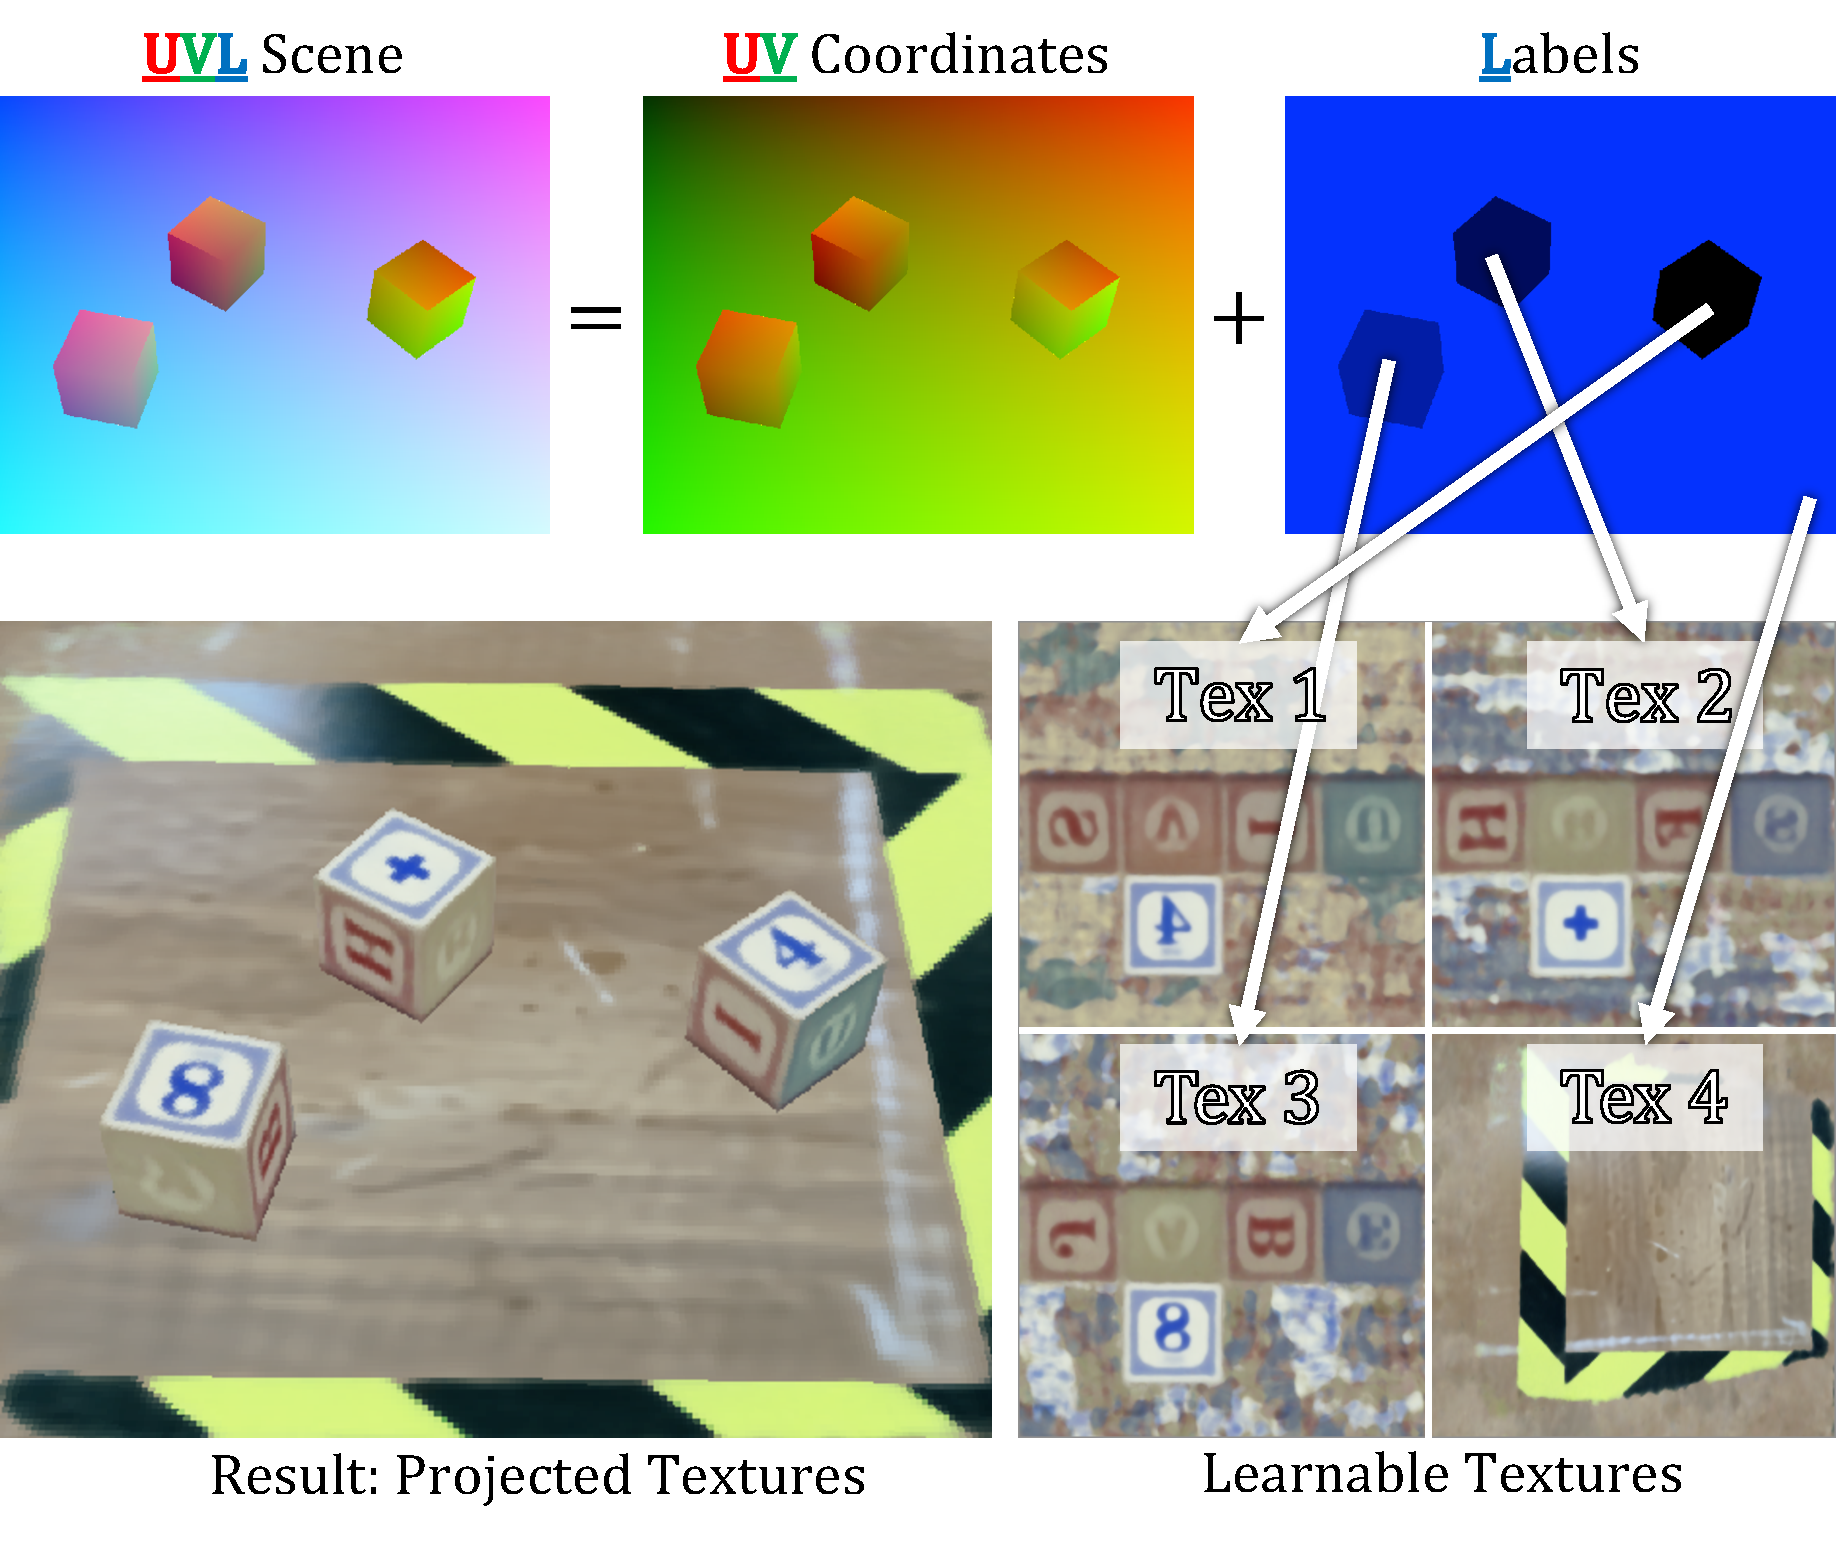
\includegraphics[width=270pt]{uvl_explanation.pdf}
	\end{center}
	\caption{
		This diagram shows the purpose of a UVL image.
		 A UVL scene is an image that has three channels: RGB.
		 R and G are used for U and V, and B is used for L.
		 L stands for Label, and determines which part of the synthetic image will get which texture.
		 The U and V coordinates correspond to positions on each texture,
		 	telling it how to project the textures onto the 3d objects represented in the UVL scene.
		The darkest shade of blue corresponds to the 1st texture, and the next darkest shade of blue corresponds to the 2nd texture etc.
		}
	\label{fig:uvl_explanation}
\end{figure}

In this paper, we'll mostly focus on a dataset that involves three alphabet blocks that are moved across a table.
Alphabet blocks were chosen because they all have the same geometry (a cube), but have very distinct semantic textures that will make temporal inconsistency obvious to the human eye.
This dataset is analagous to data that would be collected for a third-person robotic grasping task.
However, other objects (such as cans of soda, apples, cloves of garlic etc) are also for generating other results in this paper. ((TODO: Detail the five object tests and five cube tests and other stuff like shiny cans etc)).

There are two components to this dataset: Simulated data in the form of UVL scenes, and photographs.
The camera in the simulation is positioned in approximately the same place as the real camera, with approximately the same field of view.
In both domains of this dataset, the camera never moves. Instead, the objects are randomly positioned and rotated on the table.
In both the simulation and in real life, these objects are randomly translated along the x and y axis of the table, as well as rotated on the z axis.

There are 200 photographs in this datset, and they are recorded as RGB jpg images.
There are 3000 synthetic images in this dataset, in the form of UVL images.
These UVL images are also encoded as RGB images, but provide information about the geometry of a scene.
UVL images are composed of both a UV map and a label map, and are summarized in figure \ref{fig:uvl_explanation}.
To avoid positional rounding errors, UVL images are encoded as EXR files: an image format that supports floating point values.

%===============================================================================


%===============================================================================

\clearpage
% The acknowledgments are automatically included only in the final and preprint versions of the paper.

%===============================================================================

% no \bibliographystyle is required, since the corl style is automatically used.
\bibliography{example}  % .bib

\end{document}
